%! TEX program = xelatex
\documentclass[tikz]{standalone}
\usepackage[lining]{ebgaramond}
\usepackage[math-style=ISO, bold-style=ISO]{unicode-math}
\setmathfont{Garamond-Math.otf}
\begin{document}
  \begin{tikzpicture}[fill=white]
    \node at (0,0) {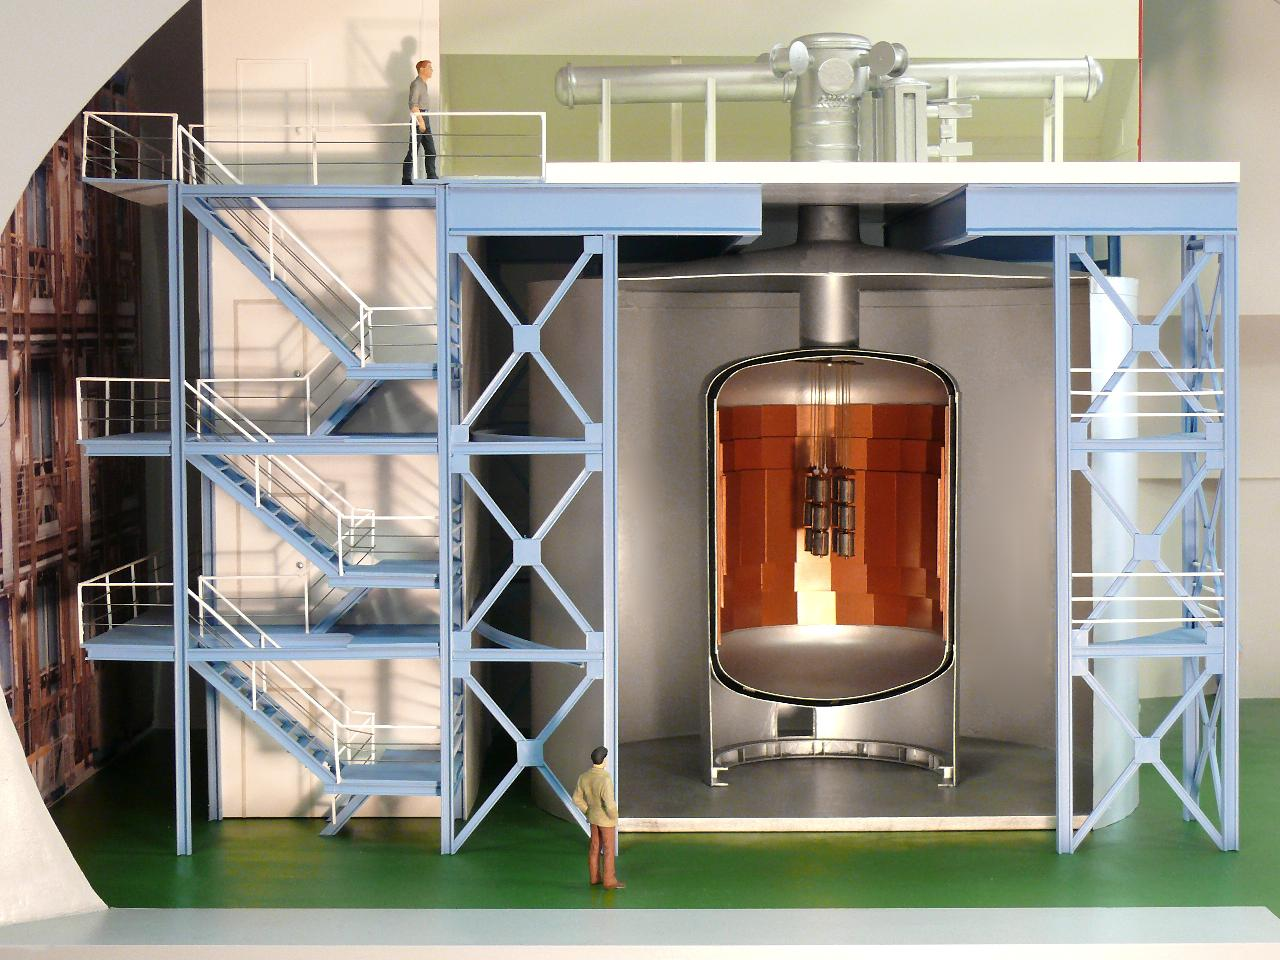
\includegraphics[height=7cm]{gerda-artist.jpg}};
    \node(e) at (3.5,3.3) [rectangle,draw,fill] {\textsc{scintillators}};
    \draw[thick,red,->] (e.south) .. controls +(0,-1) and +(0,1) .. (2.3,2.4);
    \node(a) at (1.6,-1.2) [rectangle,draw,fill] {LAr};
    \node(b) at (3.2,1.6) [rectangle,draw,fill] {$^{76}$Ge \textsc{detectors}};
    \draw[thick,red,->] (b.south) .. controls +(0,0) and +(1,0) .. (1.9,-0.4);
    \node(c) at (-1.5,1.6) [rectangle,draw,fill] {H$_2$O};
    \draw[thick,red,->] (c.south) .. controls +(0,0) and +(-1,0) .. (0,-1);
    \node(d) at (0,3) [rectangle,draw,fill] {Cu \textsc{shielding}};
    \draw[thick,red,->] (d.south) .. controls +(0,0) and +(-1,0) .. (1,0);
    \node at (-1.5,-3.15) [rectangle,draw,fill] {\small Laboratori Nazionali del Gran Sasso (LNGS)};
    \node at (7.5,0) {\includegraphics[height=7cm]{gerda-lngs.jpg}};
  \end{tikzpicture}
\end{document}
